\begin{figure}[H]
\centering
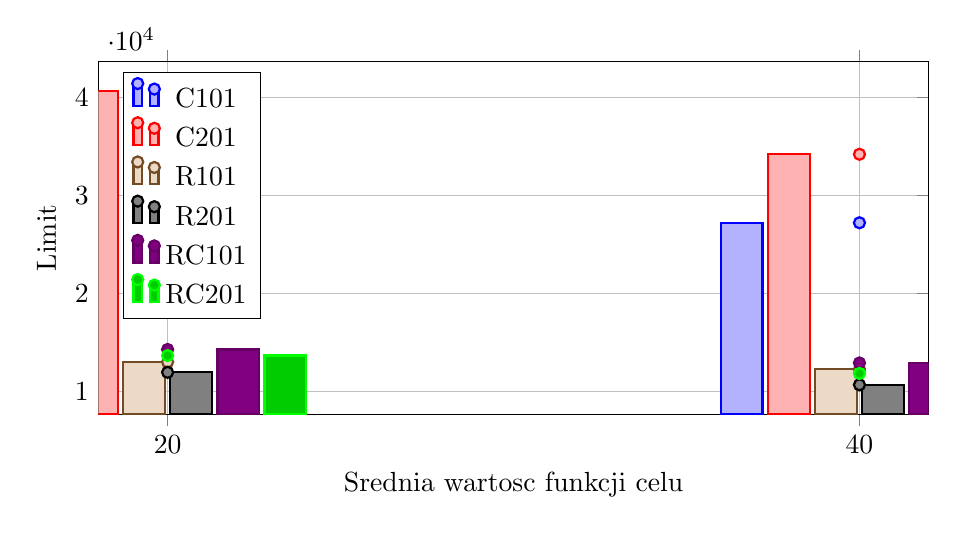
\begin{tikzpicture}
\begin{axis}[
xlabel = {Srednia wartosc funkcji celu},
ylabel = {Limit},
legend pos = north west,
grid = both,
width=1\linewidth,
height=0.5\linewidth,
ybar,
bar width=15pt,
symbolic x coords={20,40,},
xtick=data
]
\addplot + [mark = *, thick] coordinates
    {
(20,30793.0)(40,27234.083333333332)};
\addlegendentry
{C101}
\addplot + [mark = *, thick] coordinates
    {
(20,40697.0)(40,34219.75)};
\addlegendentry
{C201}
\addplot + [mark = *, thick] coordinates
    {
(20,13041.583333333334)(40,12294.916666666666)};
\addlegendentry
{R101}
\addplot + [mark = *, thick] coordinates
    {
(20,11984.0)(40,10712.666666666666)};
\addlegendentry
{R201}
\addplot + [mark = *, thick] coordinates
    {
(20,14313.5)(40,12939.0)};
\addlegendentry
{RC101}
\addplot + [mark = *, thick] coordinates
    {
(20,13689.666666666666)(40,11864.333333333334)};
\addlegendentry
{RC201}
\end{axis}
\end{tikzpicture}
\caption
{Srednia wartosc funkcji celu w zaleznosci od limitu dla poszczegolnych instancji}
\label{fig:mean_goals_per_limit_per_instance}
\end{figure}
